\subsection{JAM based on surface brightness} \label{sec:results_JAM_SB}

In this section we create dynamical models for J1331 following the procedure in Section \ref{sec:model_JAM}. We use the deprojected surface brightness MGE from Table \ref{tab:MGEF814W} for the tracer distribution $\nu(R,z)$ and to generate mass models $\rho(R,z)$. The only exception is the first test, where the mass model comes from lensing constraints.

\paragraph{JAM with lens mass model.} We make an independent prediction for the $v_\text{rms}$ curve by evaluating Equation \Wilma{[TO DO]} (with $\beta_z = 0$) for the lens mass model in Table \ref{tab:bestfitlensmodel} ($\alpha = 1$, flat rotation curve). In addition, we also calculate a  $v_\text{rms}$ curve for a lens model which was found analogously, but assumed a slightly rising rotation curve slope of $\alpha=1.1$. The predictions are compared with the data in Figure \ref{fig:JAM_modelL}. The agreement within $R' \sim 3''$ is striking: The $\alpha > 1$ model recreates the observed central dip, while the $\alpha = 1$ model fits the wings around $R_\text{eff}$. This is in concordance with observations in other galaxies. For $R'> R_\text{eff}$ we would expect $\alpha<1$. Our lensing model assumes $\alpha(R')=\text{const}$, although Figure \ref{fig:JAM_modelL} suggests, that a model with variable $\alpha(R')$ might fit even better, and maybe also reproduce the sharp drop in $v_\text{rms}$ around $R' \sim 3''$. We note however, that the most reliable constraint is around $R_\text{ein}$. Outside of $R_\text{ein}$ lensing models are only extrapolations.

%==================================================================

\begin{figure}
  \centering
  \includegraphics[height=6cm]{fig/lensing_JAM_comparision.ps}
  \caption{Comparison (not a fit!) of the symmetrized stellar $v_\text{rms}$ data of J1331 (blue dots) with JAM models generated from mass distributions which were independently derived from lensing constraints in Section \ref{sec:results_lensing}. \Wilma{[TO DO: Add Note that outside Rein extrapolation.]} The red solid line corresponds to the lens model for a flat rotation curve ($\alpha = 1$) in Table \ref{tab:bestfitlensmodel}; the green line is a best fit lens model found analogously from the image positions, but for a fixed rotation curve slope of $\alpha = 1.1$. For the JAM modelling a best fit MGE to the lens mass models were used, as well as the observed surface brightness MGE in Table \ref{tab:MGEF814W}, assuming velocity isotropy $\beta_z = 0$ and an inclination of $i = 70^\circ$.The red and black dotted lines are the Einstein radius and the effective half-light radius, respectively.}
  \label{fig:JAM_modelL}
\end{figure}

%==================================================================

%==================================================================

\begin{figure}
  \centering
  \includegraphics[height=6cm]{fig/jam_A2_vrms.ps}
  \caption{Comparison of the symmetrized $v_\text{rms}$ data of J1331 (blue dots) with a best fit dynamical JAM model (solid red line) assuming mass-follows-light and with two free parameters: $\Upsilon_\text{I,tot}^\text{dyn}$, the total I-band mass-to-light ratio found from dynamics, which converts the observed surface brightness in Table \ref{tab:MGEF814W} into a mass distribution, and the velocity anisotropy parameter $\beta_z$. The ``best'' fit is $\Upsilon_\text{I,tot}^\text{dyn} = 4.8 \pm 0.1$ and $\beta_z = -0.5$, where the latter is however pegged at the lower limit of the allowed value range. This is obviously not a good model.}
  \label{fig:JAM_modelA2}
\end{figure}

%==================================================================


\paragraph{JAM with "mass-follows-light" and velocity anisotropy.} The first JAM model that we fit to the observed $v_\text{rms}$ within $R'<5''$ is a mass-follows-light model. Mass-follows-light models are often used in dynamical JAM modelling (e.g., \citealt{GlennEC,Cap06}) and generate a mass distribution by multiplying the intrinsic light distribution $\nu(R,z)$ by a constant total mass-to-light ratio  $\Upsilon_\text{I,tot}^\text{dyn}$. This assumes that the DM is always a constant fraction of the total matter distribution within the region covered by the kinematics. This simplified mass model sometimes gives good representations of the inner parts of galaxies, where the stellar component dominates.

We also allow for a overall constant but non-zero velocity anisotropy $\beta_z$ in the model. The model parameters ($\Upsilon_\text{I,tot}^\text{dyn},\beta_z$) that fit the $v_\text{rms}$ data best are found using a $\chi^2$-fit and are demonstrated in Figure \ref{fig:JAM_modelA2}. 

For $\beta_z$ we imposed the fitting limits $\beta_z \in [-0.5,+0.5]$. While the outer parts of galaxies often show radially biased velocity anisotropy up to $\sim 0.5$ (from dynamical modelling of observed elliptical galaxies, e.g., \citet{Kronawitter2000}) and cosmological simulations (e.g., \citealt{2004MNRAS.352..535D,2001ApJ...557..533F}), the centers of galaxies are near-isotropic or have negative velocity anisotropy \citep{2003ApJ...583...92G}. Only in extreme models (e.g., around in-spiralling supermassive black holes, e.g., \citealt{1997NewA....2..533Q}) velocity anisotropies as low as $\sim -1$ have been found.

%==================================================================

\begin{figure*}
\centering
\begin{subfigure}{.5\textwidth}
  \centering
  \includegraphics[height=6cm]{fig/jam_G_vrms.ps}
  \caption{Comparison of $v_\text{rms}$ data and best fit model.}
  \label{fig:JAM_modelG}
\end{subfigure}%
\begin{subfigure}{.5\textwidth}
  \centering
  \includegraphics[height=6cm]{fig/jam_G_enclMass.ps}
  \caption{Projected local mass-to-light ratio profile and enclosed mass.}
  \label{fig:enclMass_modelG}
\end{subfigure}
\caption{JAM model found by fitting an increasing total mass-to-light ratio $\Upsilon_\text{I,tot}(R')$ profile used to generate a mass model from the light distribution.  This is done by assigning a different mass-to-light ratio to each Gaussian in the MGE in Table \ref{tab:MGEF814W}. \emph{Panel (a):} Comparison between the stellar $v_\text{rms}$ data (blue points) and the best fit model (green line). \emph{Panel (b):} Projected mass-to-light profile $\Upsilon_\text{I,tot}(R')$ along the major axis (blue line, left axis) of the best fit model. The best fit mass-to-light ratios of the first four Gaussians are plotted against each Gaussians $\sigma$ (yellow stars). The two Gaussians with the largest $\sigma$ (the fifth is not shown) have the same best fit mass-to-light ratio. Shown is also the enclosed mass inside the projected radius $R'$ on the sky (green line, right axis). The enclosed mass curve is overplotted with the independent finding for the Einstein mass $\pm 4 \%$ in Table \ref{tab:bestfitlensmodel} (red dot) at the Einstein radius (red dotted line). Shown is also the effective half-light ratio $R_\text{eff}$ (black dotted line). \Wilma{[TO DO: Mention second axis only after 1st axis is explained.]}}
\label{fig:modelG}
\end{figure*}

%==================================================================

The best fit in Figure \ref{fig:JAM_modelA2} however strives to very negative $\beta_z$ to be able to reproduce the deep central dip in the  $v_\text{rms}$ curve.\footnote{Without limiting the fitting range, the best fit would be a unrealistically low $\beta_z \sim -2$.} But $\beta_z = -0.5$ is not even a remotely agreeable fit and lower anisotropies are not to be expected or realistic. We also tested radial profiles for $\beta_z(R)$ of the form proposed by \citet{BaesVanHese}, which was however equally unable to reproduce the data. We conclude, that this is due to the well-known degeneracy between anisotropy and mass profile \Wilma{[TO DO: REF]} and the mass-follows-light model is \emph{not} a good representation of the mass distribution in J1331's inner regions.

\Wilma{[TO DO: Make sure that we explain somewhere, why we model only in the inner regions]}

\paragraph{JAM with increasing mass-to-light ratio.} In Section \ref{sec:results_lensing} we found from lensing constraints, that the light distribution might drop faster with radius than the mass distribution. This could correspond to a radially increasing total mass-to-light ratio. As velocity anisotropy alone cannot explain the observed kinematics in a simple a mass-follows-light model, we now allow for a mass-to-light ratio gradient in the JAM modelling. We therefore generate a mass model from the light distribution in Table \ref{tab:MGEF814W} by assigning each of the five Gaussians in the MGE its own total mass-to-light ratio $\Upsilon_{\text{I,tot,}i}$ and replace the total luminosity in Equation \eqref{eq:centralItotalL} $L_i$ with the Gaussians total Mass $M_i = \Upsilon_{\text{I,tot,}i} L_i$. We treat the five $\Upsilon_{\text{I,tot,}i}$ as free fit parameters and only require that $\Upsilon_{\text{I,tot,}j} \geq \Upsilon_{\text{I,tot,}i}$ when the corresponding $\sigma_j \geq \sigma_i$ to ensure that the overall mass-to-light ratio is increasing with radius.

Figure \ref{fig:enclMass_modelG} shows the best fit (projected local) mass-to-light ratio profile, which rises from $\Upsilon_\text{I,tot} = 2.53$ in the center and approaches a value of $\Upsilon_\text{I,tot} = 7.60$ outside of the fitted region at $R'\gtrsim 3''$. The central mass-to-light ratio is in agreement with the mass-to-light ratio $\Upsilon_\text{I,*}^\text{chab} = 2.5 \pm 0.6$, given in Table \ref{tab:previousresults} based on the results of \citet{SWELLSI} assuming a stellar population with a \citet{Chabrier2003} IMF (see also Section \ref{sec:MLdiscussion}). When assuming that galaxy bulges are in general older and redder in the center \Wilma{[TO DO: REF]}, i.e., $\Upsilon_\text{I,*}$ is more likely to drop with radius than to rise, the strong increase of $\Upsilon_\text{I,tot}(R')$ might be due to a strong contribution of dark matter in J1331.

Figure \ref{fig:JAM_modelG} shows that the best fit model nicely reproduces the central dip in the $v_\text{rms}$ curve, even though it has difficulties fitting the drop around $R' \sim 4''$. The latter might be because we only allowed the $\Upsilon_\text{I,tot}(R')$ to rise. A slight drop could be expected when the reddish bulge turns into the bluish disk and the contribution of the stellar component becomes less due to a lower $\Upsilon_\text{I,*}$ for younger and bluer populations.

In Figure \ref{fig:enclMass_modelG} we overplot the enclosed mass profile with the Einstein mass $M_\text{ein} = (7.77 \pm 0.33) \cdot 10^{10} M_\odot$ at the Einstein radius found from lensing in Table \ref{tab:bestfitlensmodel}. The agreement between the Einstein mass and the independently found $M(<R_\text{ein}) = 7.49 \cdot 10^{10} M_\odot$ from dynamical modelling is striking.
